%--------------------------------------------------
%	Chapter 5. GNN Pattern Recognition Algorithm
%--------------------------------------------------

\chapter{Graph Neural Network Pattern Recognition Algorithm}\label{chapter-5}

Once compatible hit-pairs have been established, they can be used to build a graph network to represent a particle collision event. This chapter presents a novel pattern recognition algorithm utilising GNN architectures to prune connections in such a network, in order to reconstruct tracks in a silicon based Pixel detector. The application is focused on the Pixel detector, with the aim that the approach will serve as a sophisticated track seeding technique for Pixel hits and form preliminary track candidates. These seeds can be extended into the Strips using standard track following. Such an approach could be efficient for saving computational resources if the GNN does not produce large proportions of fake tracks. The ultimate aim of this work is to develop a realistic algorithm for fast track reconstruction that can be deployed in future high-luminosity phases of particle detector experiments. This research was presented at the 2022 Connecting the Dots (CTD) conference at the University of Princeton USA and is currently under review for publication in the Springer Journal: Computing for Software and Big Science \cite{Lad_2023_gnn}. Sections \ref{gnn-algorithm-overview} to \ref{gnn-kf-implementation} presents an overview and detailed breakdown of each stage of the algorithm. Section \ref{gnn-application-toy-model} illustrates a simple application on a toy model.



\section{Algorithm Overview}
\label{gnn-algorithm-overview}
The GNN based pattern recognition algorithm is considered an iterative mixture reduction task, which allows the deactivation of incompatible connections (GNN edges termed as outliers) in order to improve track parameter estimates and iteratively extract track candidates. 

Individual hits or clusters of hits are modelled as graph nodes and track segments are modelled as graph edges. Once the graph network is constructed, each edge is modelled as a Gaussian state in order to approximate the local track state probability density. Therefore, each node is initialised with a Gaussian mixture of track states, local to its neighbourhood of connections.

After initialisation, the network evolves iteratively, where an iteration is made up of three main stages illustrated in Figure \ref{fig:flowchart}. The first stage comprises of Gaussian Mixture Reduction (GMR). This involves a traditional ML approach, whereby compatible Gaussian states are grouped together using clustering techniques and outlier states can be identified. This stage is followed by information aggregation by leveraging message passing between nodes in a given neighbourhood. The compatibility of neighbouring states can be assessed via extrapolation, in order to improve local track parameters using neighbourhood information. The third stage involves updating the network state at each node, as certain connections are deactivated. A graph splitting algorithm is also applied directly after the first two stages to identify good track candidates, and if discovered they are extracted. 

Unlike traditional methodologies whereby Multi-Layered Perceptrons (MLPs) are employed for deep learning strategies, the proposed GNN leverages simplified KFs embedded in the network and are used for two main purposes. Firstly, the KF is used as a mechanism for information propagation, in order to iteratively improve the precision of track parameters. The KF is also used in extraction of track candidates compatible with particle motion model. This allows the model to efficiently exploit a prior knowledge about charged particle dynamics as the network evolves.

The excitation and inhibition rules of individual edge connections are designed to facilitate the “simple-to-complex” approach for “hits-to-tracks” association, such that the network starts with low hit density regions of an event and gradually progresses towards more complex areas. As the network evolves, the uncertainty in local track orientation decreases until there are no more track candidates that fulfil the criteria for a good track. This is the end state of the network where isolated nodes, track fragments and unresolved ambiguities will remain.

\begin{figure}[htbp]
    \centering
    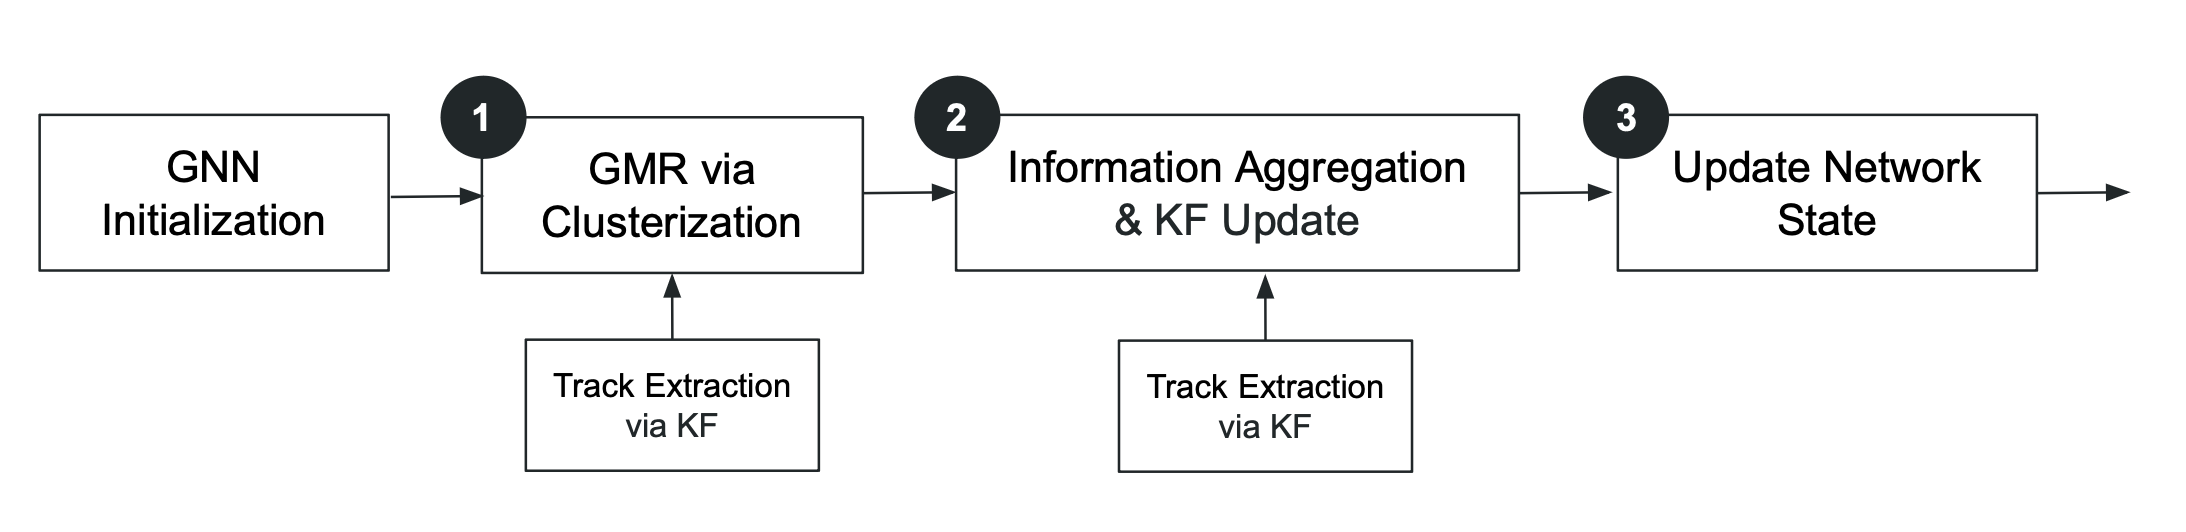
\includegraphics[width=0.98\textwidth]{images/5-gnn-algorithm/gnn-workflow.png}
    \caption{Flow chart illustrating all stages making up an iteration of the GNN-based algorithm. After each stage, a Kalman filter (KF) is applied in order to iteratively extract candidates. After stage three, a further Gaussian Mixture Reduction (GMR) stage would be applied repeating the iterations.}
    \label{fig:flowchart}%
\end{figure}



\section{Graph Network Initialization}
\label{gnn-network-initialization}

The graph network is constructed using the Python library \textit{NetworkX} \cite{SciPyProceedings_11}. Hits from a particle event are represented as nodes and predicted hit-pairs as edge connections. See chapter \ref{chapter-4} for further details on the hit-pair predictor used to form edge connections. Following this, a common computer vision technique, known as Connected Component Analysis (CCA), is applied using a built-in function\cite{networkx}. CCA detects connected regions in data structures and allows the network to be split into smaller, more manageable graphs referred to as \textit{subgraphs}. 

Each pairwise connection between node $i$ and neighbour node $j$ forms a Gaussian state, $X_{ij}$, representing the local track parameter estimate. Each edge has an associated prior probability $p_{ij}$ and edge weight $w_{ij}$. The prior probability of node $i$ and neighbour node $j$ belonging to the same track is determined, assuming a track can produce at most one hit per layer of the detector. $w_{ij}$ is a mixture weight for the compatibility of the Gaussian state transmitted from node $i$ to neighbour node $j$, representing the strength of the connection. $w_{ij}$ are initialised as uniform dependent on the number of neighbours local to a node and are updated based on how the network evolves. $w_{ij}$ are not to be confused with the traditional weights associated to features within neural networks.

A Gaussian mixture, $g_i(X)$, is formed from weighted Gaussian components, $\phi_{ij}$, at node $i$, which describes the local neighbourhood and is given by Eq \eqref{eqn:gaussian-mixture},

\begin{equation}
g_i(X) = \sum_{j} w_{ij}\phi_{ij}(X, X_{ij}, C_{ij})
\label{eqn:gaussian-mixture}
\end{equation}

where $C_{ij}$ are the edge state covariances. All edges act as bidirectional conduits, such that message passing can occur in both directions. All edges are initialised as \textit{active}, allowing the propagation of state information, whereas \textit{deactive} edges are defined to not allow state information to be propagated. 

%Figure \ref{fig:network-initial} illustrates a node and its neighbourhood.

% \begin{figure}[htbp]%
%     \centering
%     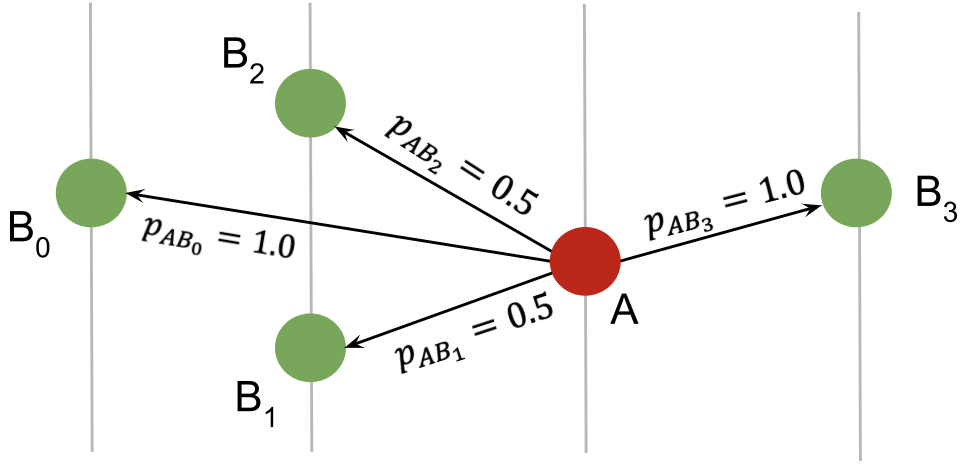
\includegraphics[width=8.8cm]{images/5-gnn-algorithm/network-initialisation.png}%
%     \caption{Prior probabilities associated to network edges of node A's local neighbourhood. Neighbours $B_j$ are located on separate detector layers shown by vertical lines. The unidirectional edges indicate the direction of propagation of state information and priors. These entities will differ from nodes $B_j$ distributing messages to their corresponding neighbourhoods.}%
%     \label{fig:network-initial}%
%\end{figure}



\subsection{Constructing Track State Estimates}
\label{constructing-track-states}

Track parameters in both the transverse $x$-$y$ plane and the $r$-$z$ plane are considered in order to construct track state estimates $X_{ij}$.

\subsubsection{Parabolic Model}
\label{parabolic-state}

In the $x$-$y$ plane, charged particles experience the influence of the magnetic field, so naturally their trajectories follow a near-parabolic shape. For a given node A, a parabola is formed using the origin O, node A and neighbour node B, illustrated in Figure \ref{fig:gnn-parabolic-model}. The parabola is transformed into the local coordinate system of node A such that the new $x$-axis, $X_A$ goes through the global origin O and node A. The parabolic parameters \{$a, b, c$\} are computed using equations Eq \eqref{eqn:parabolic-equations}. The measurement vector $[m_O \quad m_A \quad m_C]$ is obtained in the coordinate system local to node A, assuming $m_O = 0$ and $m_A = 0$.

\begin{equation}
\begin{aligned}
m_O = ax_{O}^{2} + bx_O + c \\
m_A = c \\
m_B = ax_{B}^{2} + bx_B + c
\end{aligned}
\label{eqn:parabolic-equations}
\end{equation}

\begin{figure}[htbp!] 
    \centering
    \subfloat[]{%
        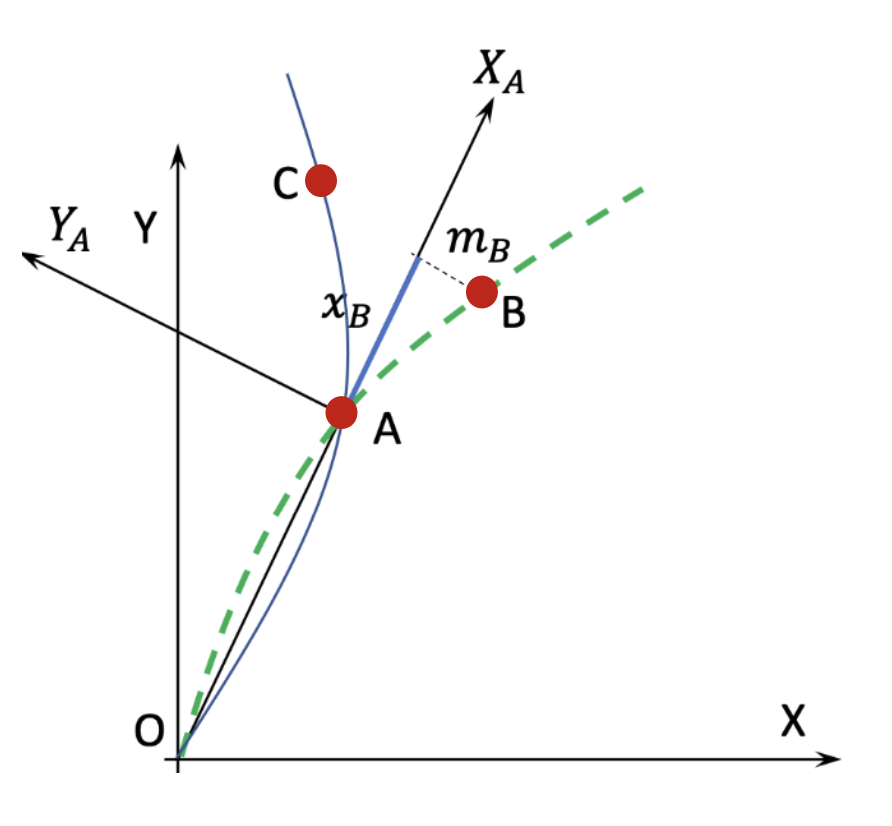
\includegraphics[width=0.43\textwidth]{images/5-gnn-algorithm/parabolic-state-model-1.png}%
        \label{fig:gnn-parabolic-state-1}%
        }%
    \hfill%
    \subfloat[]{%
        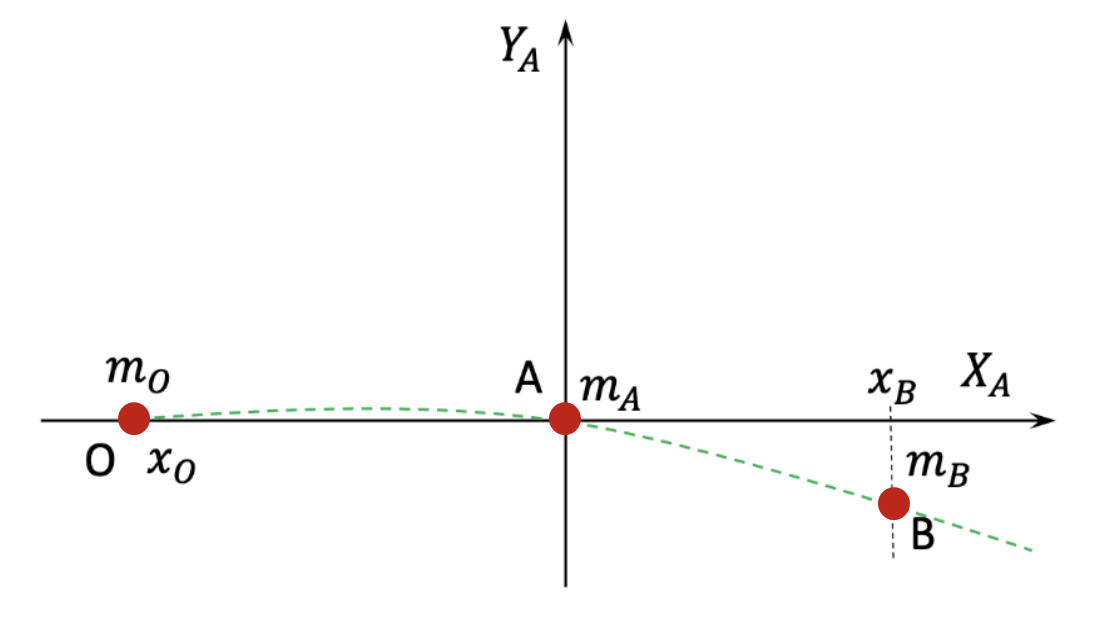
\includegraphics[width=0.57\textwidth]{images/5-gnn-algorithm/parabolic-state-model-2.png}%
        \label{fig:gnn-parabolic-state-2}%
        }%
    \caption{Illustrations of the parabolic model used in the $x$-$y$ plane. a) shows the construction of a parabola between the global origin, O and nodes A - B, as well as a second parabola between O - A - C. b) shows the rotation of the parabola O - A - B into the local coordinate system of node A.}
    \label{fig:gnn-parabolic-model}
\end{figure}


\subsubsection{Linear Model}
\label{linear-state}

The $r$-$z$ plane is parallel to the direction of travel of the beamline, where tracks follow a linear model. The inverse track inclination between a node and its neighbour, $\tau$, is used and is given by Eq \eqref{eqn:tau-parameter}, where $z_A$, $r_A$ refer to measurements of the node and $z_B$, $r_B$ refer to measurements of its neighbour. $r$ is the square root of the sum in quadrature of the $x$ and $y$ measurements.

\begin{equation}
\tau = \frac{z_A - z_B}{r_A - r_B}
\label{eqn:tau-parameter}
\end{equation}

% \begin{figure}[htbp]%
%     \centering
%     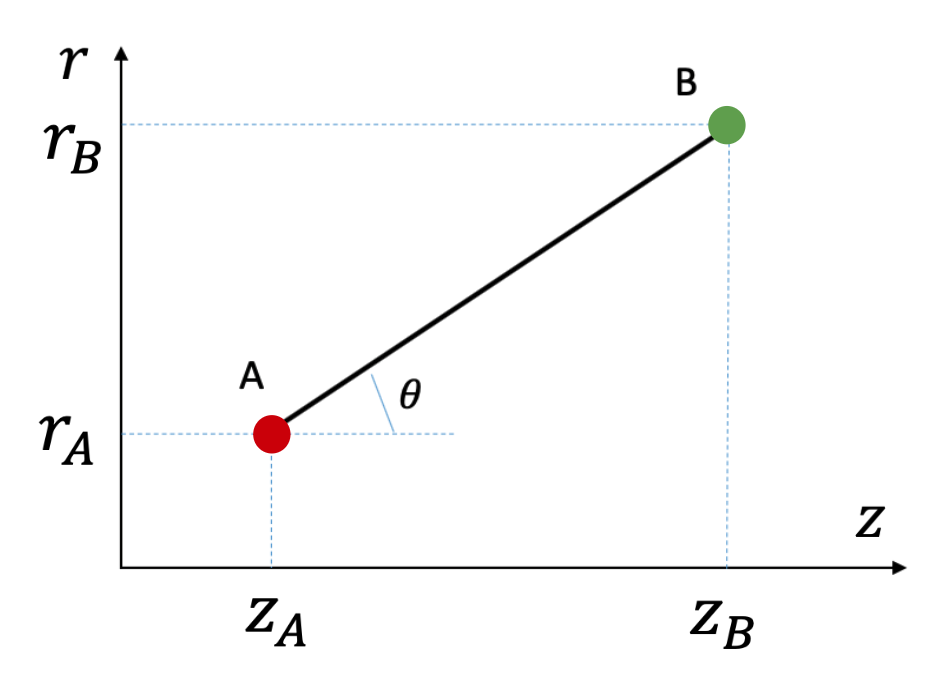
\includegraphics[width=0.45\linewidth]{images/5-gnn-algorithm/linear-state-model.png}%
%     \caption{Edge connection between nodes A and B in the $r$-$z$ plane, where $\theta$ is the angle of inclination from the $z$ axis to the A-B edge.}%
%     \label{fig:linear-state-model}%
% \end{figure}


\subsubsection{Track State Estimate}

Parabolic parameters $a$ and $b$ in the $x$-$y$ plane, as well as inverse track inclination $\tau$ in the $r$-$z$ plane give an indication of track orientation. For node $i$ and its neighbour $j$, the track state estimate $X_{ij}$ is given by Eq \eqref{eqn:joint-state-vector}

\begin{equation}
X_{ij} = \begin{bmatrix} a \\ b \\ \tau \end{bmatrix}
\label{eqn:joint-state-vector}
\end{equation}


\subsubsection{Derivation of State Covariance}



\subsubsection{Molière Theory of Multiple Scattering}
\begin{itemize}
\item highland formula and handling the error/effects due to multiple scattering for the barrel and endcap in slightly different ways
\item how were the covariances dervied and the sigma errors chosen
\item Derivation of the edge state covariance
\item 2 different ones, we start with the edge covariance, and derive the state covariance
\end{itemize}
% moliere theory links:
%https://gray.mgh.harvard.edu/attachments/article/337/Techniques%20of%20Proton%20Radiotherapy%20(06)%20Multiple%20Scattering.pdf
%https://pdg.lbl.gov/2005/reviews/passagerpp.pdf





\section{Gaussian Mixture Reduction}
For nodes with a high multiplicity of edge connections, the number of track states can quickly rise. To make inferences within a reasonable amount of processing time, GMR is used to prevent the number of components from exploding. One computationally efficient approach for GMR is a clustering-based algorithm. A high order Gaussian mixture is approximated by one with lower order, using the traditional k-means clustering \cite{kmeans}. At each node, similar track states are clustered together forming a reduced mixture and their corresponding edges remain active, illustrated in Figure \ref{fig:GMR-example}. A single merged state estimate $X_{M}$ and merged state covariance $C_{M}$ is formed from the clustered states, using the inverse-variance weighting \cite{inverse-variance-weighting}. Simultaneously, states that are not clustered are identified as outliers and deactivated.

\begin{figure}[htbp!] 
    \centering
    \subfloat[]{%
        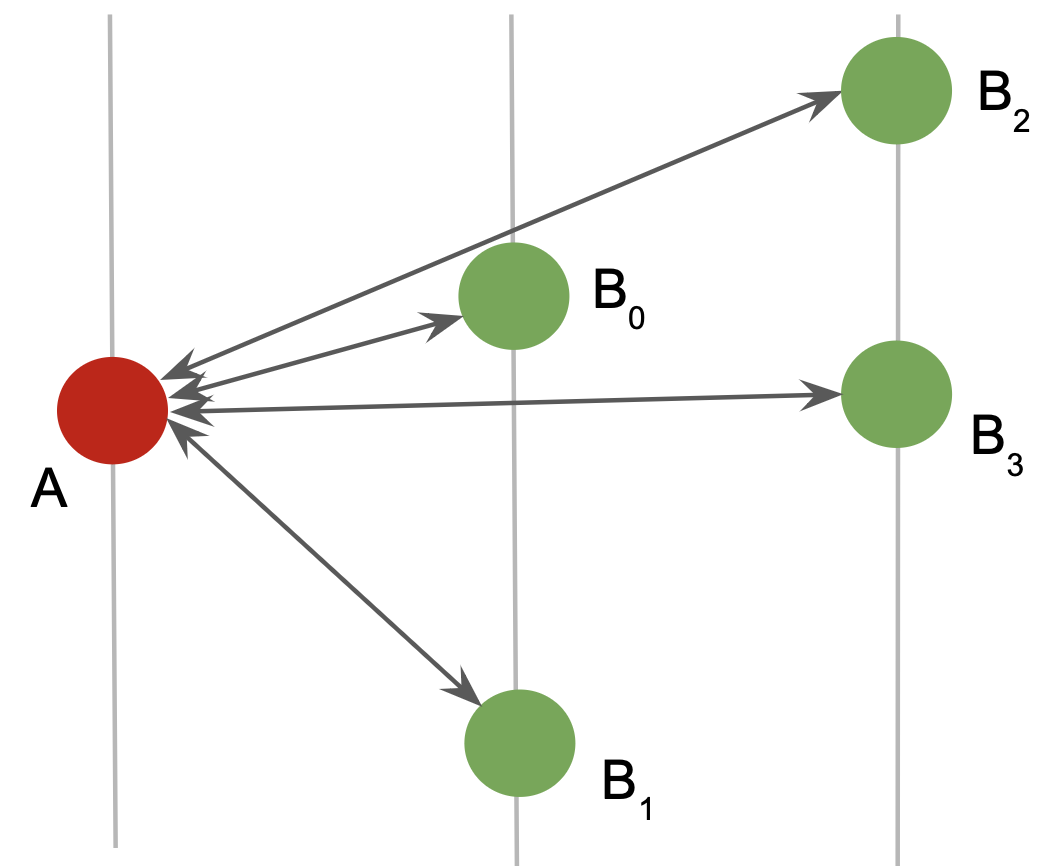
\includegraphics[width=0.43\linewidth]{images/5-gnn-algorithm/GMR-1.png}%
        \label{fig:GMR-1}%
        }%
    \hfill%
    \subfloat[]{%
        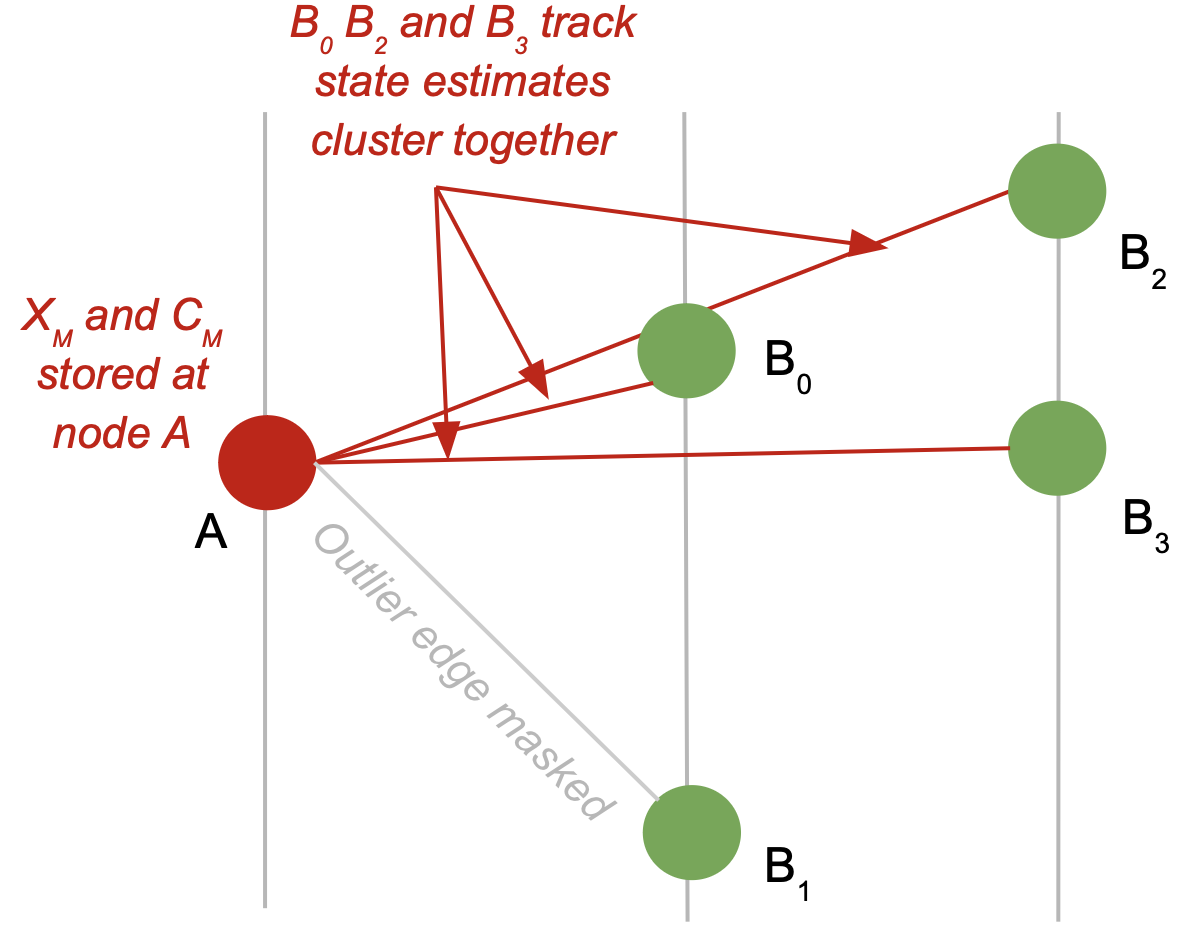
\includegraphics[width=0.57\linewidth]{images/5-gnn-algorithm/GMR-2.png}%
        \label{fig:GMR-2}%
        }%
    \caption{GMR via clustering applied to graph networks, with the aim of identifying incompatible edge connections. a) shows node $A$ and its local neighbourhood $B_j$. b) shows the expected result of GMR applied to all track state estimates local to node $A$, where an outlier edge $A - B_1$ has been deactivated. A merged track state $X_M$ is formed from states $X_{AB_0}$, $X_{AB_2}$, $X_{AB_3}$ and the corresponding merged state covariance $C_M$ is formed from $C_{AB_0}$, $C_{AB_2}$, $C_{AB_3}$.}
    \label{fig:GMR-example}
\end{figure}

The k-means clustering is implemented using the general case of $k=1$ to model the Gaussian mixture at each node as a single track alongside outlier connections. For the case where a graph node is located in close proximity to an intersection point between two tracks, two or more clusters of states can be expected. In such a case, the mixture reduction process is declared impossible and all track states are propagated to later stages for further processing. This part of the graph network will remain dormant until competing edges are deactivated and the mixture becomes more unimodal. 


\subsection{The Kullback-Leibler Threshold}
%In order to establish whether clustering of track state estimates is feasible for a given node, a deviation measure is needed to serve as a threshold. 
The Kullback-Leibler (KL) divergence, $d_{KL}$, is a measure of the statistical distance between two Gaussian probability distributions \cite{KL, FRUHWIRTH19971} and is used as a threshold to determine when track states can be grouped together into a cluster. The $d_{KL}$ between $X_{ij}$ and $X_{ik}$ is given by Eq \eqref{eqn:kullback-leibler}, where $G_{ij}$ = $C_{ij}^{-1}$.

\begin{equation}
    d_{KL} = tr[(C_{ij} - C_{ik})(G_{ij} - G_{ik})] + (X_{ij} - X_{ik})^{T}(G_{ij} + G_{ik})(X_{ij} - X_{ik})
    \label{eqn:kullback-leibler}
\end{equation}

The optimal $d_{KL}$ threshold will differ for each node depending on its local neighbourhood. For example, consider a node with a high variance of edge orientation in its neighbour connections, $\sigma_{e}$. The corresponding $d_{KL}$ threshold will be larger in comparison to a node with a small $\sigma_{e}$. 

To determine the optimal pairwise $d_{KL}$, a MC simulation of $10,000$ particle collision events, each event with ten truth tracks, was used to build a training dataset. Loosely compatible edge connections were formed using a hit-pair predictor based on track inclination angle of neighbouring hits. The feature vector was comprised of $\sigma_{e}$ for a given node, and pairwise $d_{KL}$ between track states. The ground truth particle was extracted for each pairwise connection, where truth 1 corresponded to hits from both track states originating from the same truth particle, and truth 0 otherwise. A SVM was trained to discriminate between the two classes \cite{scikit-learn}, using a polynomial degree three kernel. Predictions were adjusted such that the TPR was tuned to 95\% and the decision boundary was converted into a fast LUT using a similar methodology outlined in Section \ref{LUT-generation}. 

% Other classification algorithms were explored, however the SVM was the most appropriate classifier to determine a decision boundary to best separate the classes.

\begin{figure}[htbp!] 
    \centering
    \subfloat[]{%
        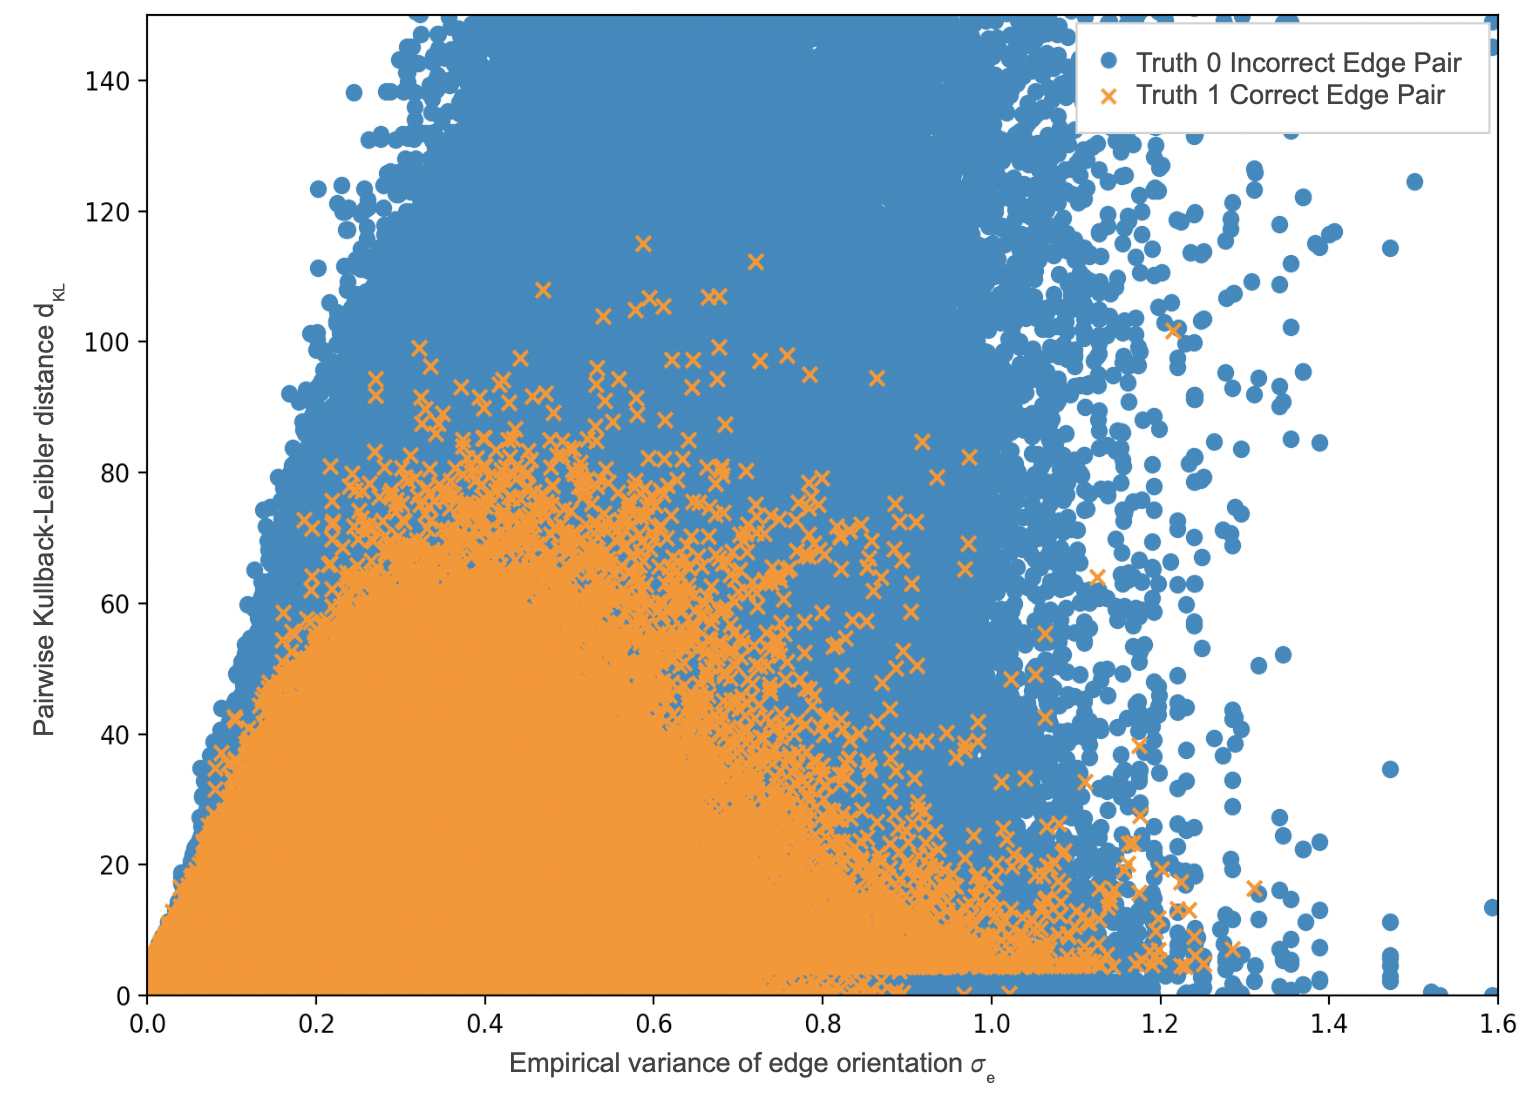
\includegraphics[width=0.8\linewidth]{images/5-gnn-algorithm/kl-truth.png}%
        \label{fig:KL-distance-truth}%
        }%
    \hfill%
    \subfloat[]{%
        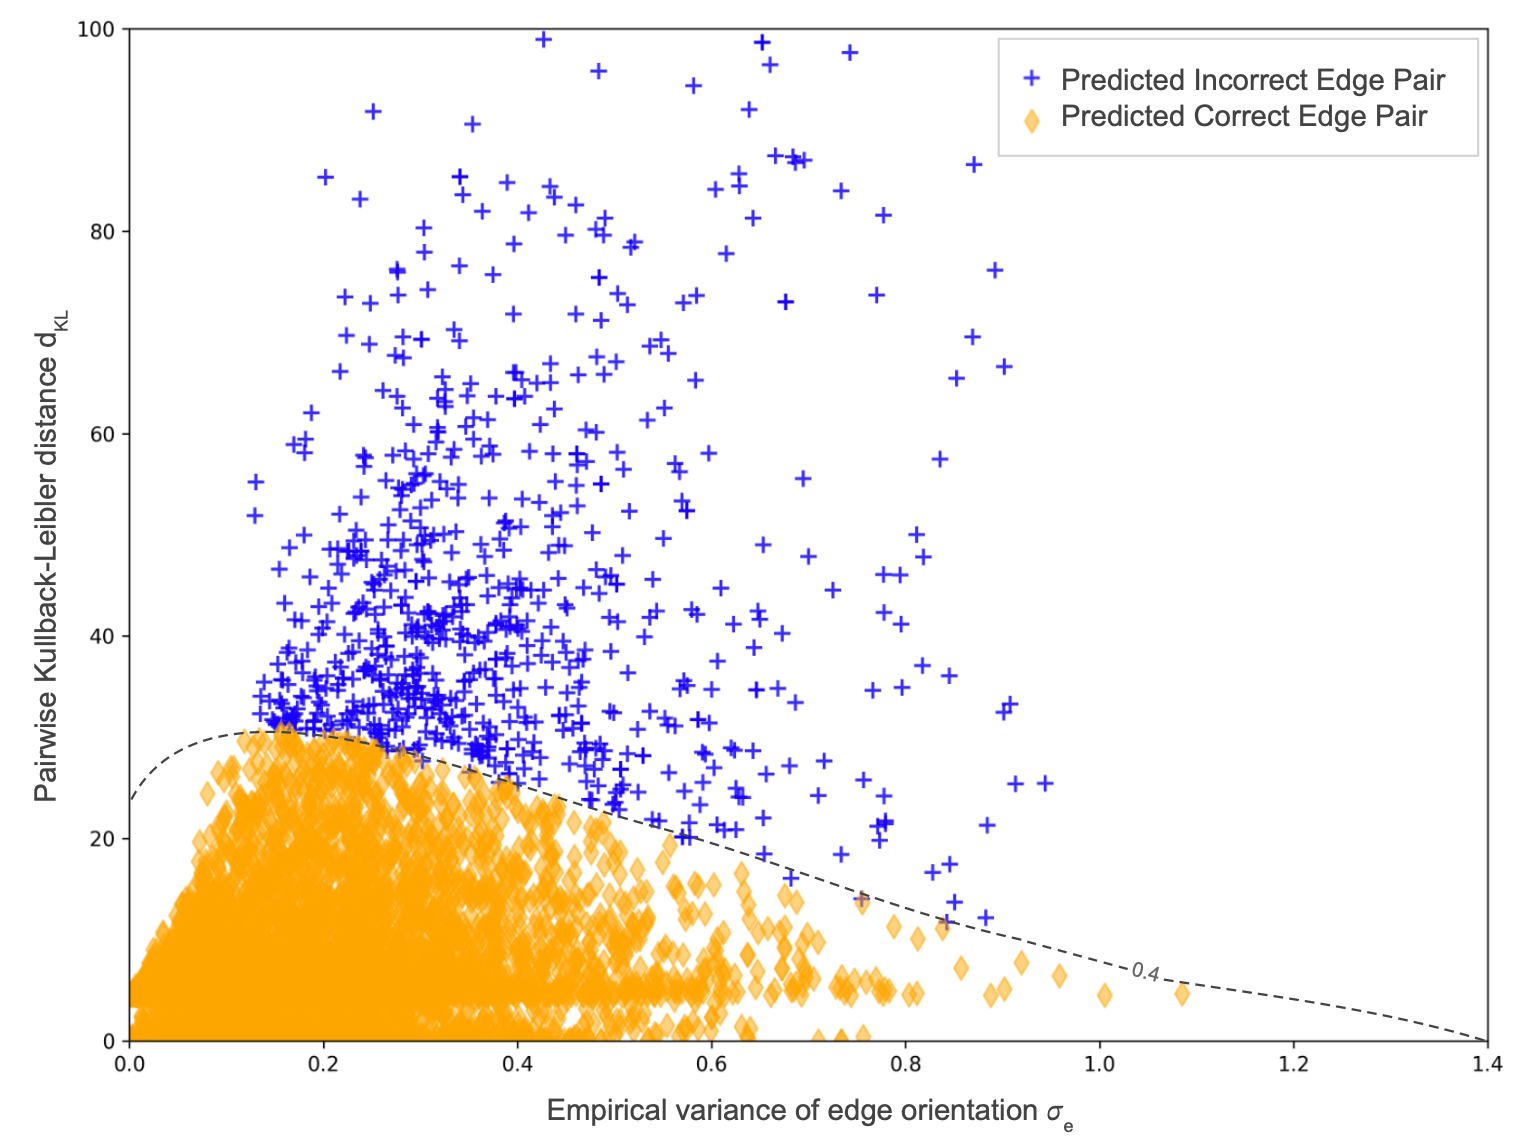
\includegraphics[width=0.8\linewidth]{images/5-gnn-algorithm/kl-predictions.png}%
        \label{fig:KL-distance-predictions}%
        }%
    \caption{}
    \label{fig:KL-distance}
\end{figure}






\section{Information Aggregation}
% As the mixture is reduced, $X_{ij}^{M}$ and $C_{ij}^{M}$ are of higher precision and are propagated to further stages of the algorithm.

%Neighbourhood information aggregation via message passing is a key feature within graph networks and is leveraged within the second stage of the GNN-based algorithm. 

%Bidrectional message passing ensures that the compatibility of any state propagated can be assessed in both directions, dependent on a node's local neighbourhood. and ensures the compatibility of propagated states can be assessed in both directions.

At each node, information is propagated to neighbouring nodes for all active edge connections. Once these neighbours obtain information from their own neighbours, state extrapolation and validation is executed. 

At each node, the track state is represented by a Gaussian mixture, or a reduced mixture (the merged state ($g_i(X)$). As illustrated in Figure \ref{fig:extrapolation} for a given node $i$, if the merged state was established in the previous stage, this is distributed alongside its covariance matrix to all neighbour nodes $j$. If a merged state is not available, then all track state estimates are distributed to all neighbours $j$. The parameter estimation begins with a linear projection onto the subspace of measurements. Each track state estimate is projected via a measurement matrix $H$, which relates the track state to the measurement values. In order to validate if the connection between nodes $i \rightarrow j$ is compatible, the Mahalanobis distance $\Delta \chi^{2}_{ij}$ is calculated using the residual vector between the projected state $HX$ and the measurement at the neighbour state. If $\Delta \chi^{2}_{ij}$ is below some threshold $d$, the connection is compatible and the KF update is applied. If $\Delta \chi^{2}_{ij} > d$ then the connection is deemed incompatible and deactivated. The threshold $d$ is a hyper-parameter, representing the maximum $\Delta \chi^{2}_{ij}$ acceptable.


\begin{equation}
\tilde{X}_{ij} = F_{ij} X_{ij} \qquad \tilde{C}_{ij} = F_{ij} \biggl( \sum C_{ij} + Q \biggl) F^{T}_{ij}
\label{eqn:extrapolation}
\end{equation}

\begin{figure}[htbp]
        \centering
        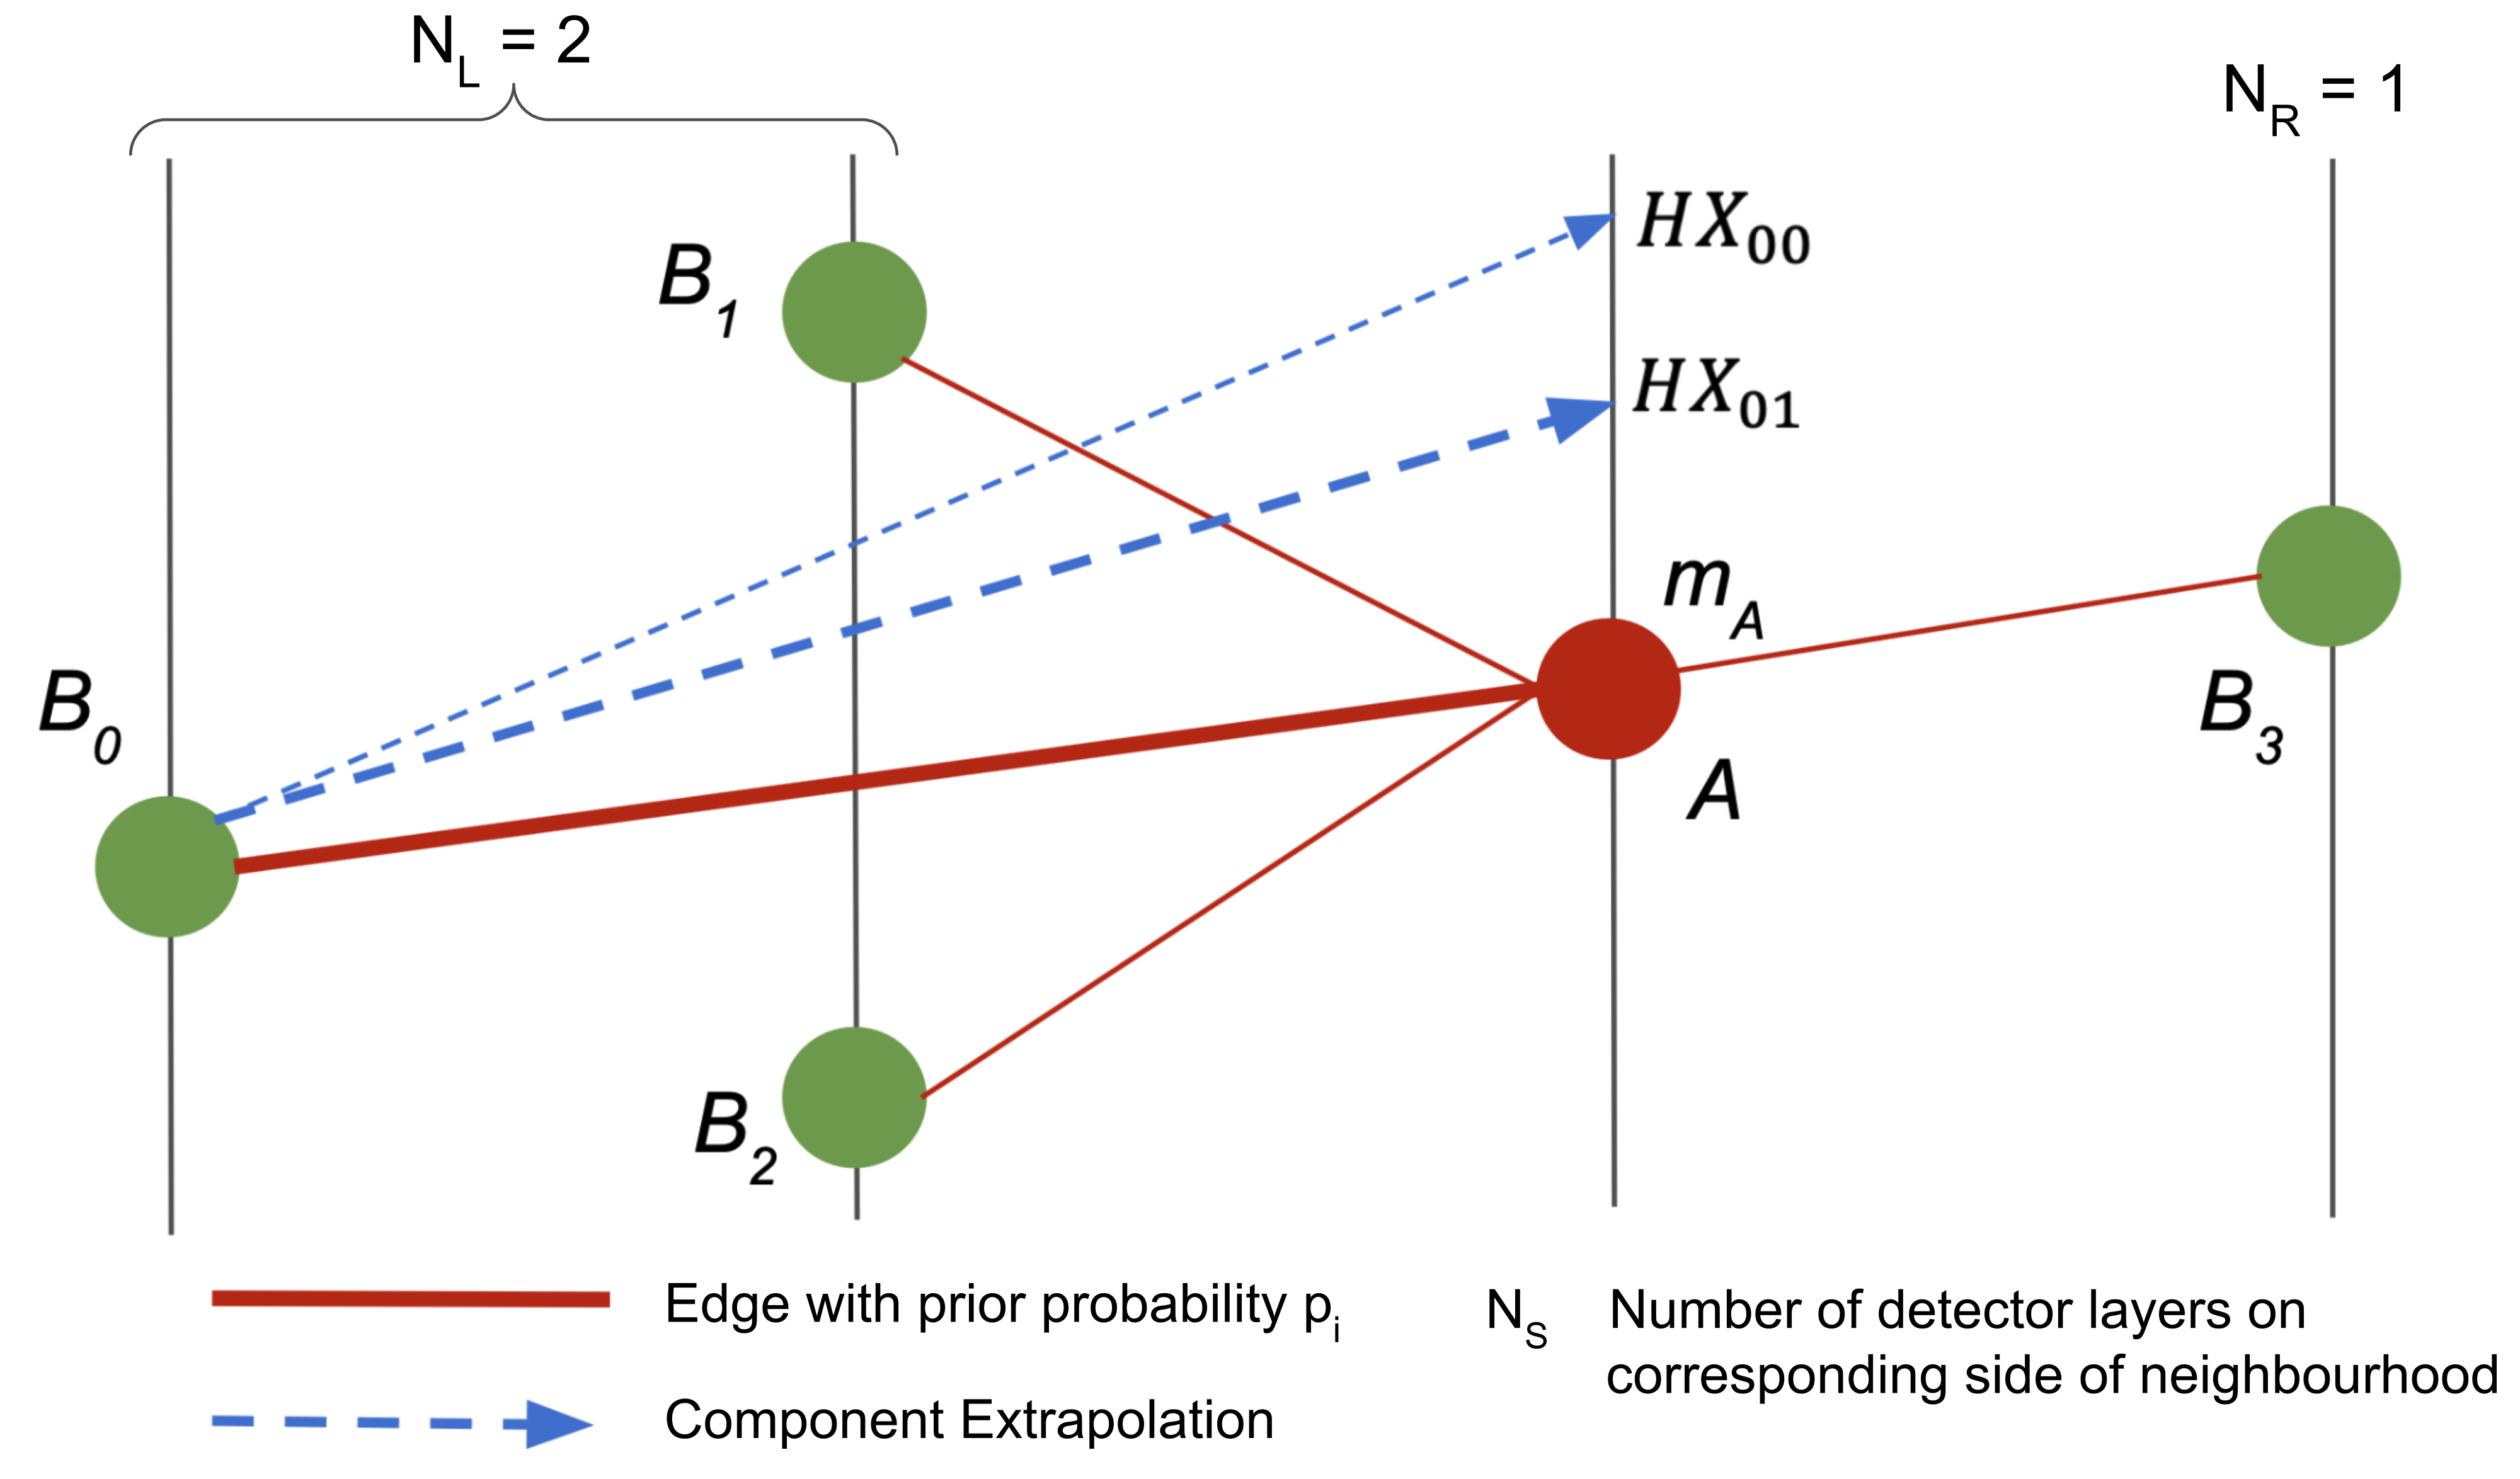
\includegraphics[width=0.85\textwidth]{images/5-gnn-algorithm/gnn-extrapolation.png}
        \caption{Track state estimates $X_{00}$ and $X_{01}$ projected from node $B_0$ to A via the measurement matrix H.}
        \label{fig:extrapolation}%
\end{figure}


\begin{itemize}
    \item Information propagation via Message Passing Mechanism
    \item Extrapolation and Validation
    \item Linear and Parabolic model - 2 different extrapolations for xy componenets of state vector and rz componenet, illustrations here
    \item Kalman Filter Update, OU process for correlated noise
\end{itemize}




\section{Updating Network State}
\label{gnn-updating-network-state}

As the network evolves and certain connections are deactivated, the local track parameter estimates for each node changes. Therefore, the corresponding edge component's $w_{ij}$ are updated. For an edge connection between nodes $i$ and $j$, the updated edge weights $\widetilde{w}_{ij}$ stated in Eq. \eqref{eqn:weights} are computed using the normalised Gaussian measurement likelihood given by Eq. \eqref{eqn:likelihood}. The denominator $\sum_{k}w_{ik}\beta_{ik}$ is the summation of the product of weights and likelihoods in a neighbourhood for a given node $i$. The updated weights $\widetilde{w}_{ij}$ are also divided by the number of detector layers on either side of its neighbourhood $N_S$, in order to account for the probability that a track passing through node $i$ was detected at layer $L$. For a given node, if any $\widetilde{w}_{ij} < 0.1$, these edge connections are automatically deactivated as the likelihood of compatibility of this incoming track state is extremely low. This forms an additional part of the mechanism for edge activation and deactivation. After this update is complete, the iterations repeat and a further GMR would be performed on updated track states. 

\begin{equation}
\beta_{ij} = (2 \pi \lvert S_{ij} \rvert )^{-1/2}  e^{-\Delta \chi^{2}_{ij} / 2}
\label{eqn:likelihood}
\end{equation}

\begin{equation}
\widetilde{w}_{ij} = \frac{1}{N_S} \frac{w_{ij}\beta_{ij} p_i}{\sum_{k}w_{ik}\beta_{ik}}
\label{eqn:weights}
\end{equation}



\section{Track Splitting and Extraction}
\begin{itemize}
    \item CCA
    \item criteria for a good track candidate
    \item Implementation of KFs/ KF track fit
\end{itemize}




\section{Application on a Simple Model}
\label{gnn-application-toy-model}

Mention here that only a linear model was used in this instance, where the track state estimate comprised of a 2x1 vector, with measurement y and inverse track inclination tau. The extrapolation and hence KR update that was used here was therefore linear too and 2x2 - will have to show a different transition Jacobian matrix.

% This indicates, that $\sigma_{e}$ is also an important feature in used as a discriminating feature when clustering. 

% TODO: mention here that the linear track state model was used and reference the section

% The excitation and inhibition rules of individual GNN nodes will be designed to facilitate the “simple-to-complex” approach for “hits-to-tracks” association, such that the network starts with relatively “easy” areas of an event (low hit density) and gradually progresses towards more complex areas (high hit density). 

% \begin{itemize}
% \item Application on a simple toy mc model and heat network - track extracted and metrics
% \end{itemize}

A 2-dimensional simulation with seven tracks, each with ten hits, was created, see Figure \ref{fig:ground-truth}. The graph network was formed using a many-to-one mapping of hits-to-nodes, where close proximity hits were merged into one node. The threshold for close proximity hits was determined by considering the distance distribution between hits located in the same layer. In order to build edge connections in the graph network and reduce all possible combinatorics between node pairs, an edge-predictor method was devised. The predictor uses a simple calculation whereby the track inclination of neighbouring nodes is calculated. If the inclination of a neighbour spanning up to two layers apart is within a particular range, then this edge is compatible and a connection is established between the nodes. The network is initialised with its corresponding track state estimates $X_{ij}$, covariance matrices $C_{ij}$ and MC truth particle.

In order to efficiently resolve ambiguities, a method was devised to automatically determine a suitable region for initiating the pattern recognition. For a given node, the variance of edge orientation $\sigma_e^2$ of its neighbourhood was considered. Figure \ref{fig:heat-map} shows a heat map, indicating ``hot'' nodes (white) which represent nodes with a high degree (number of edges associated to the node), whereas ``cold'' nodes (orange - red) indicate regions with fewer ambiguities to resolve. This indicates that the node degree is an indirect characteristic of how complex a local neighbourhood is and provides a method to determine where pattern recognition should begin on a graph network in order to resolve incompatible edge connections. Nodes with $\sigma_e^2 > 0.8$ were temporarily removed and the pattern recognition was initially applied to the remaining network.

\begin{center}
\begin{figure}[htbp]%
    \centering
    \subfloat[\centering Simulation of seven truth tracks]{{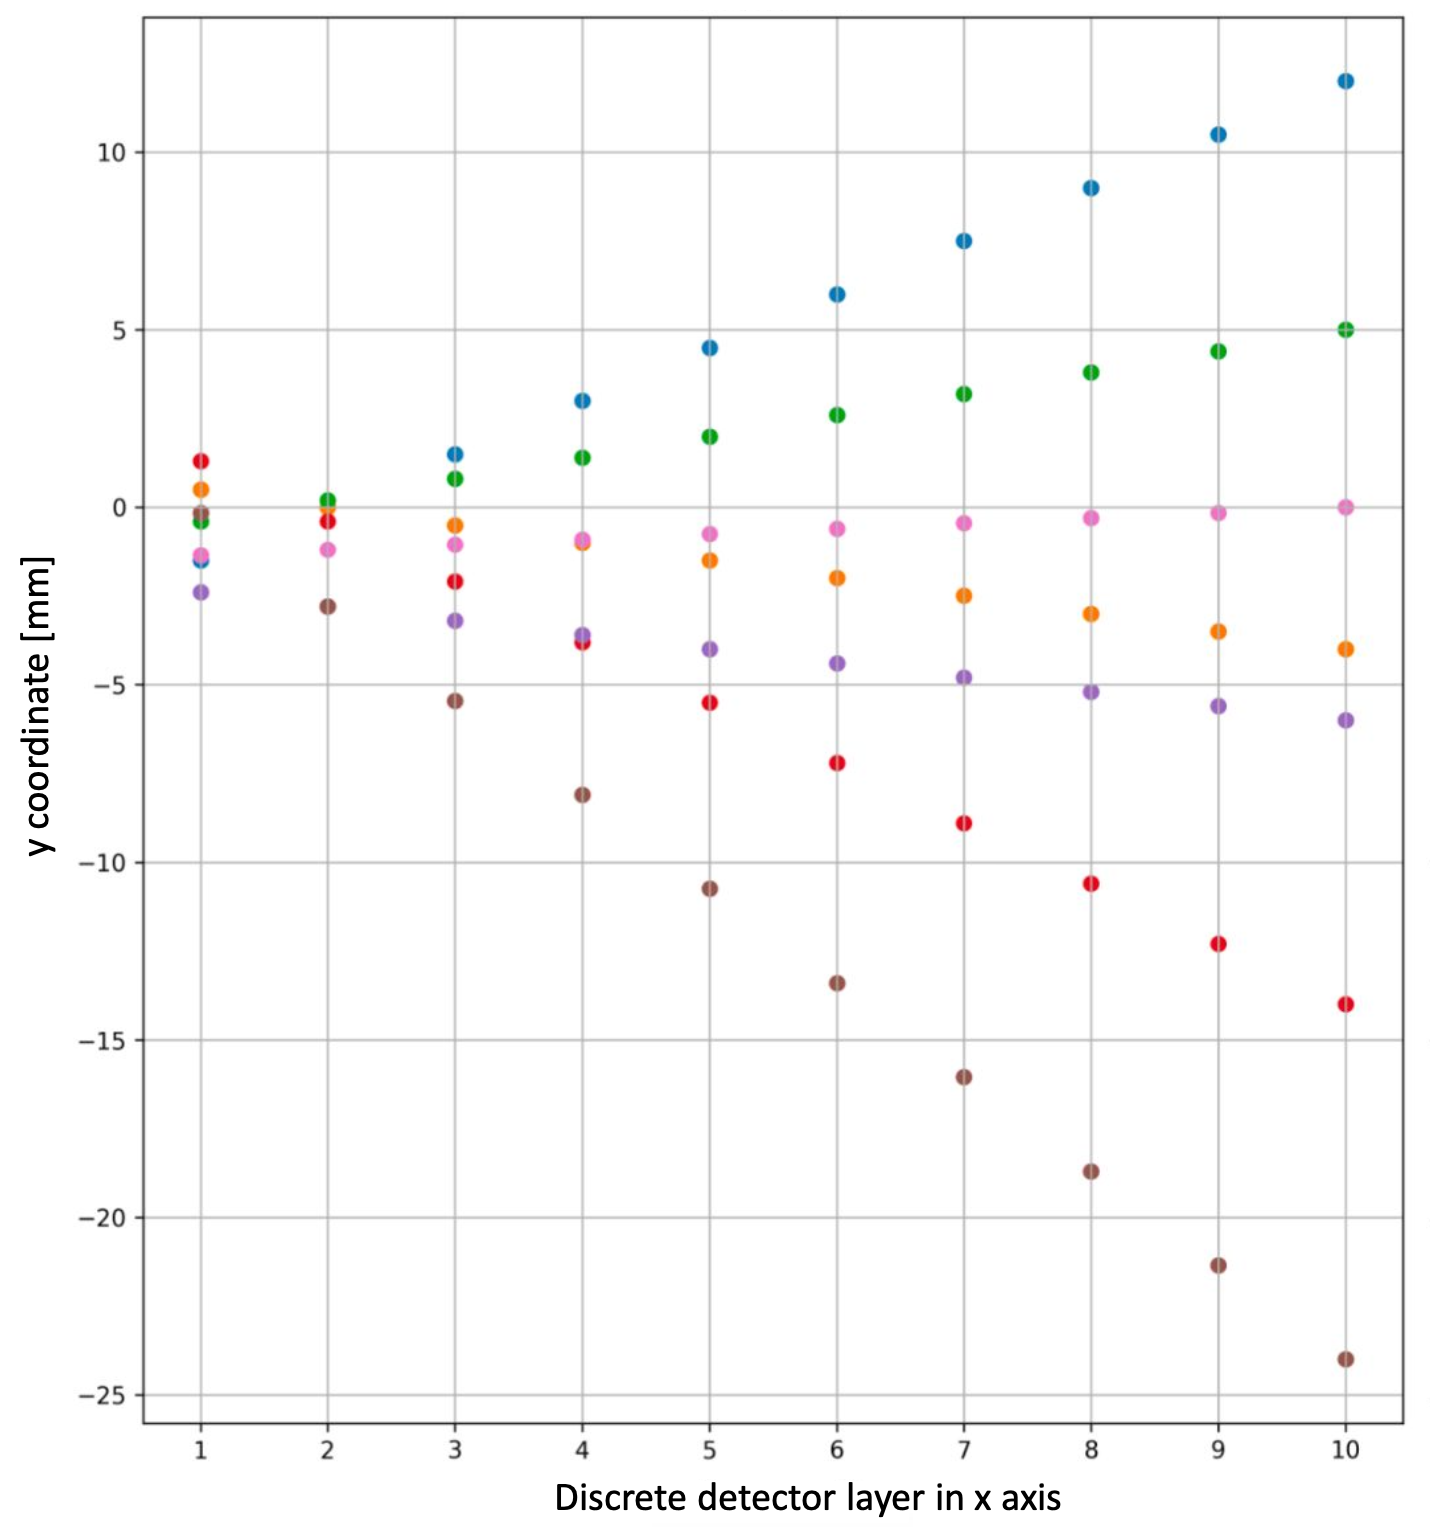
\includegraphics[width=8cm]{images/5-gnn-algorithm/ground-truth.png} } \label{fig:ground-truth}}%
    \hfill
    %\qquad
    \subfloat[\centering Graph network plotted as a node-degree heat map]{{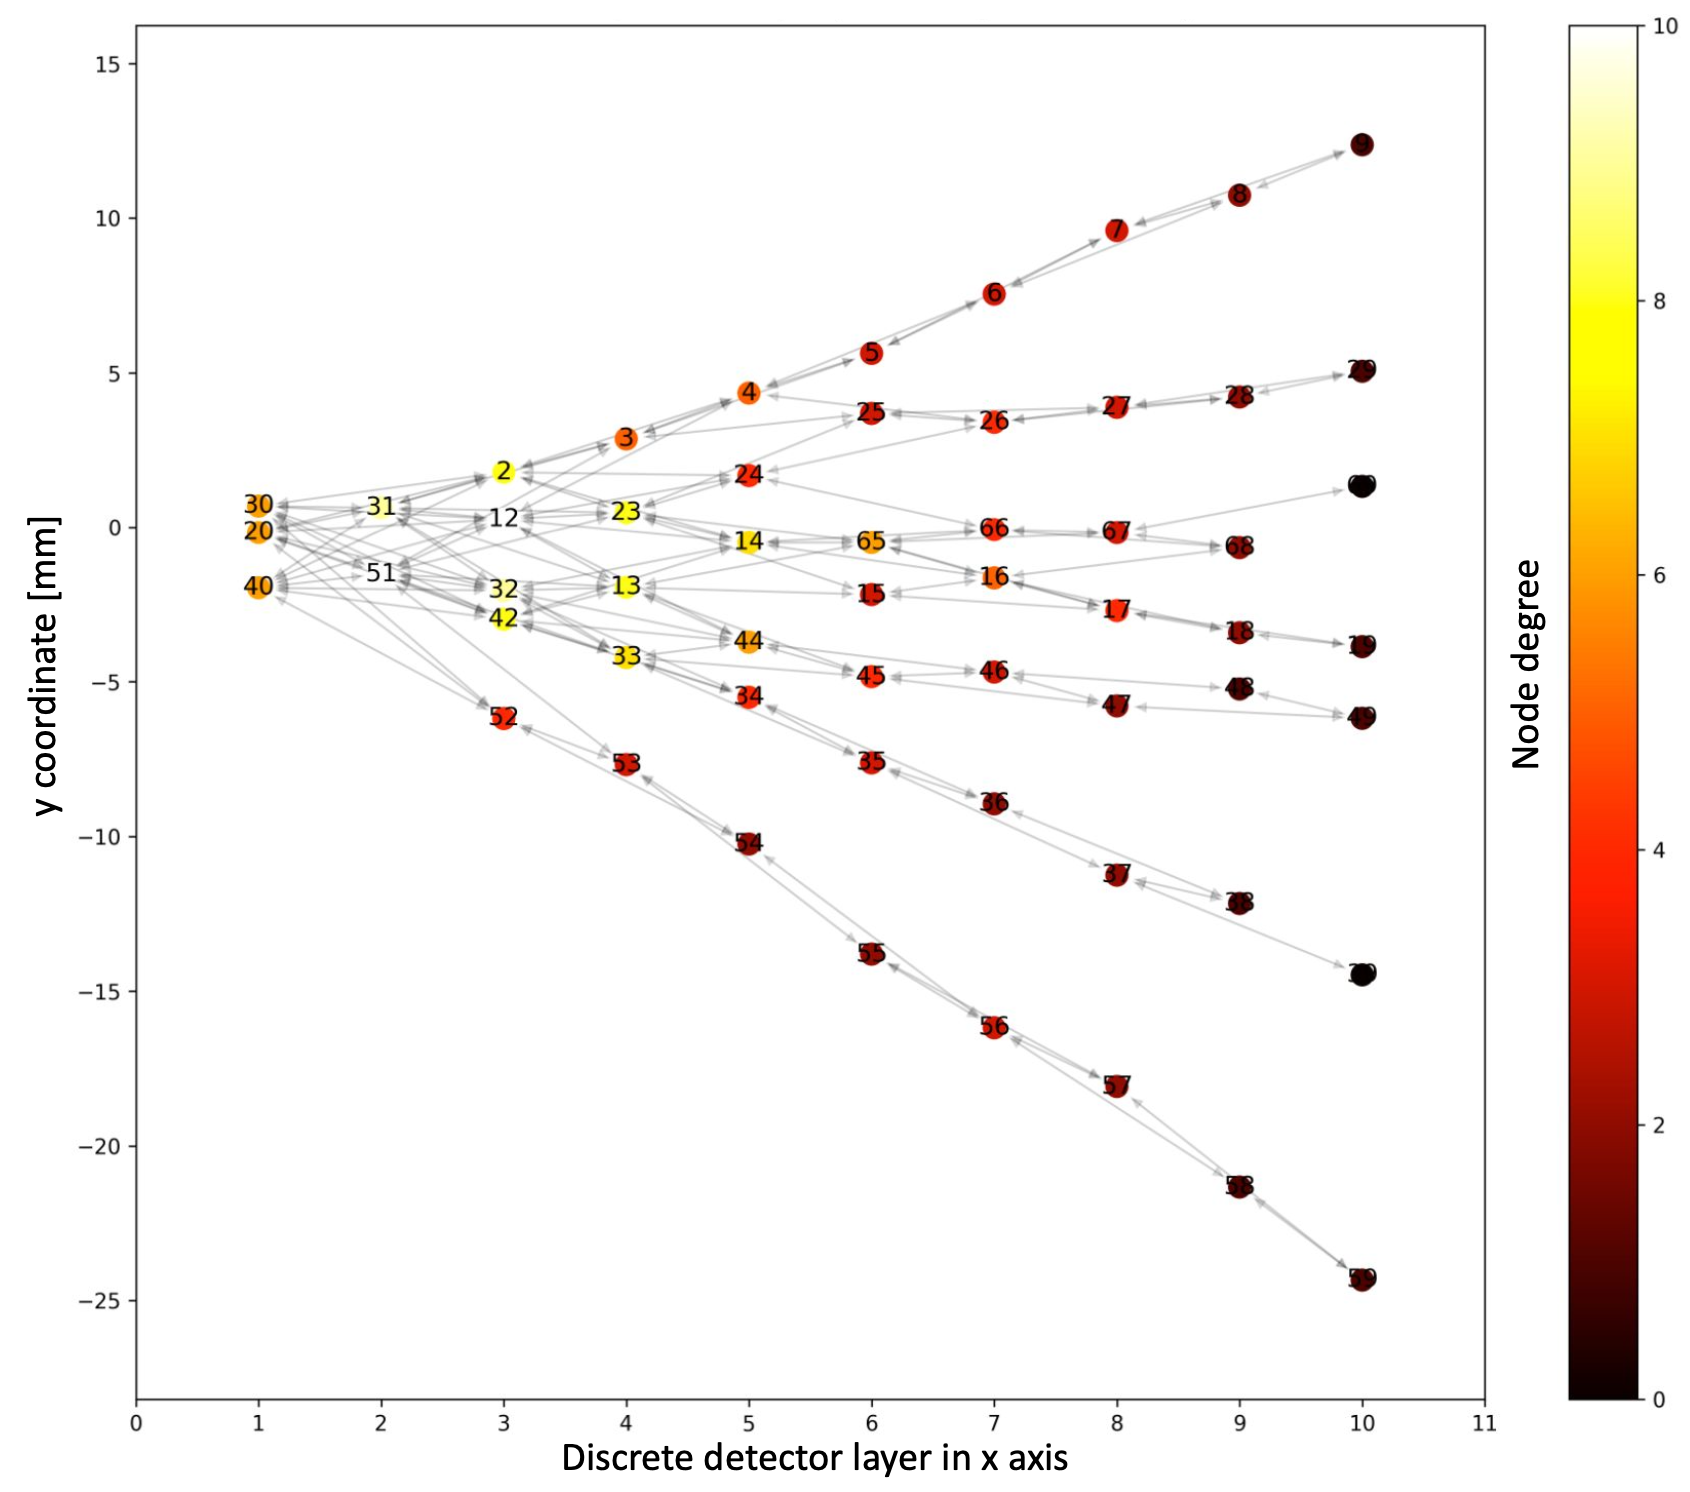
\includegraphics[width=12cm]{images/5-gnn-algorithm/heatmap-network.png} } \label{fig:heat-map}}%
    \caption{a) Simple 2-dimensional simulation of seven truth tracks where each track contains ten hits; one hit per layer. Each colour represents a different track. b)  Conversion of the simulated hits in a), to a graph network containing nodes and edges. Close proximity hits are merged into the same node where necessary and predicted edge connections are formed using a pair predictor. The heat map represents node degree, where ``hot'' nodes (white) contain many edge connections, whereas ``cold'' nodes (orange - red) contain fewer edge connections.}%
    \label{fig:setup}%
\end{figure}
\end{center}




%\section{Conclusions}
